\documentclass[preprint]{aastex} 

\usepackage[top=1in, bottom=1in, left=1in, right=1in]{geometry}
\usepackage{amsmath}
\usepackage{graphicx}
\usepackage{mdwlist}
\usepackage{natbib}
\usepackage{natbibspacing}
\setlength{\bibspacing}{0pt}
\setlength{\parskip}{0pt}
\setlength{\parsep}{0pt}
\setlength{\headsep}{0pt}
\setlength{\topskip}{0pt}
\setlength{\topmargin}{0pt}
\setlength{\topsep}{0pt}
\setlength{\partopsep}{0pt}
\setlength{\footnotesep}{8pt}
\pagestyle{empty}
\citestyle{aa}

%Project Description (8-pages maximum), including the following:
%- A statement of which of the four categories of MSIP is most appropriate
%for this proposal as the first sentence (see section II. Program Description).
%- A scientific justification. For Open Access Capabilities, explain the
%uniqueness and lack of general availability of the capability.
%- A description of the broader impacts, including student training.
%- A description of benefits to the community (observing time, data products, etc.)
%- An outline of the project management plan (where appropriate).
%Note: Results from Prior NSF Support should not be included. Links to URLs may
%not be used.

\begin{document}
%\title{Hydrogen Epoch of Reionization Arrays (HERA): From Detection to Characterization}
%\title{HERA: From Detection of Reionization to its Characterization}
\title{HERA: Characterizing Our Cosmic Dawn}
% A statement of which of the four categories of MSIP is most appropriate
%for this proposal as the first sentence (see section II. Program Description).

This proposal targets the Mid-Scale Science Projects category of the 
Mid-Scale Innovations Program solicitation.
The Hydrogen Epoch of Reionization Arrays (HERA) is a program for using the
unique capabilities of the 21cm hyperfine line to trace neutral hydrogen
through the cosmic dawn of our Universe.  The HERA roadmap submitted
to the {\it New Worlds, New Horizons of Astronomy and Astrophysics} 2010
decadal survey, (\citealt{astro2010}; hereafter NWNH) was given ``top priority in this [Radio,
Millimeter, and Sub-millimeter] category of recommended new facilities for
mid-scale funding." The HERA roadmap proceeded in three stages: HERA-IB called
for \$25M to complete the PAPER and MWA experiments; HERA-II budgeted \$62M for
an array capable of characterizing the power
spectrum of cosmic reionization in detail; HERA-III targeted 1 km$^2$ of
collecting area to image reionization structures in detail.

The PAPER and MWA experiments are now fully constructed, and will
complete their groundbreaking science program over the coming two years.
Although significantly less than \$25M was invested in HERA-IA/B, these
`spearhead projects' lead the global effort to tap the transformative
potential of the 21cm line as a probe of cosmic history.
Their greatest challenge is balancing stringent sensitivity requirements 
against the need to suppress
foregrounds that are five orders of magnitude brighter than the signal.   In
this area, there has been a major breakthrough.  Based on a new understanding
of how instrumental characteristics can be leveraged to isolate foregrounds
from the cosmological signal on the basis of spectral smoothness,
foreground emission has been suppressed by four orders of magnitude (in Jy) in PAPER
observations, down to the current sensitivity limits.
HERA-I instruments
are now sensitivity-limited, and have begun ruling out certain reionization scenarios
\citep{parsons_et_al2013}. Making the first statistical detection of 21cm
reionization remains possible at the limits of the sensitivity of current
projects.

Given this new conclusive answer to the question of how to optimize 21cm reionization
experiments for foreground removal,
the time is ripe to launch the next phase of HERA.  We propose a
staged approach to building the next-generation experiment that incorporates these
new breakthroughs, targets reionization science beyond the first detection, and
is timed to begin producing transformative science just as current HERA-I instruments
are finishing.  As described below, recent technical breakthroughs favor
larger, close-packed antenna elements, and this has substantially altered the
HERA plan.  The next step for HERA targeted in this proposal delivers the 0.1
km$^2$ collecting area and associated science of HERA-II, but 
%with less than 600 antennas, 
the improved design makes
the budget (\$16.3M), project complexity, and project team are of
a modest HERA-IB scope.
% is the budget figure too hidden?

\vspace{-0.25in}
\section{Scientific Justification}

The period beginning with the birth of the first luminous objects in the
universe, and culminating with the ionization of the intergalactic medium (IGM)
$\sim$500 Myrs later, is one of the last unexplored phases of cosmic evolution.
Exploring this epoch of reionization was highlighted as one of the three
``priority science objectives chosen by the [NWNH] survey committee for the
decade 2012-2021". Observations of Gunn-Peterson absorption
by the IGM toward the most distant quasars \citep{fan_et_al2006}, kinetic
Sunyaev-Zel'dovich features in the CMB \citep{zahn_et_al2012}, and CMB
anisotropy and polarization \citep{page_et_al2007,planck_et_al2013} indicate
that reionization was a complex process, starting perhaps as early as 
$z\approx14$, with the last vestiges of the the neutral IGM being etched away by
$z\approx6$.  Unfortunately, these ground-breaking results are limited in
diagnostic capabilities: the Gunn-Peterson effect saturates for even low
neutral fractions, and the various CMB probes provide only integral measures of 
ionization history.

Redshifted emission from the 21cm hyperfine transition of neutral hydrogen has
gained considerable attention as a unique tracer of the
primordial IGM.  Indeed, in the early universe, 21cm emission provides the
only direct probe of the complex astrophysical interplay between the first luminous
structures and their surroundings.  The direct observation of the neutral IGM via this signal
would be an achievement with a scientific payoff comparable to that of the CMB.  As
emphasized in NWNH: ``The panel concluded that to explore the
discovery area of the epoch of reionization, it is most important to develop
new capabilities to observe redshifted 21-cm HI emission, building on the
legacy of current projects and increasing sensitivity and spatial resolution to
characterize the topology of the gas at reionization."  

\begin{figure}[!ht]\centering
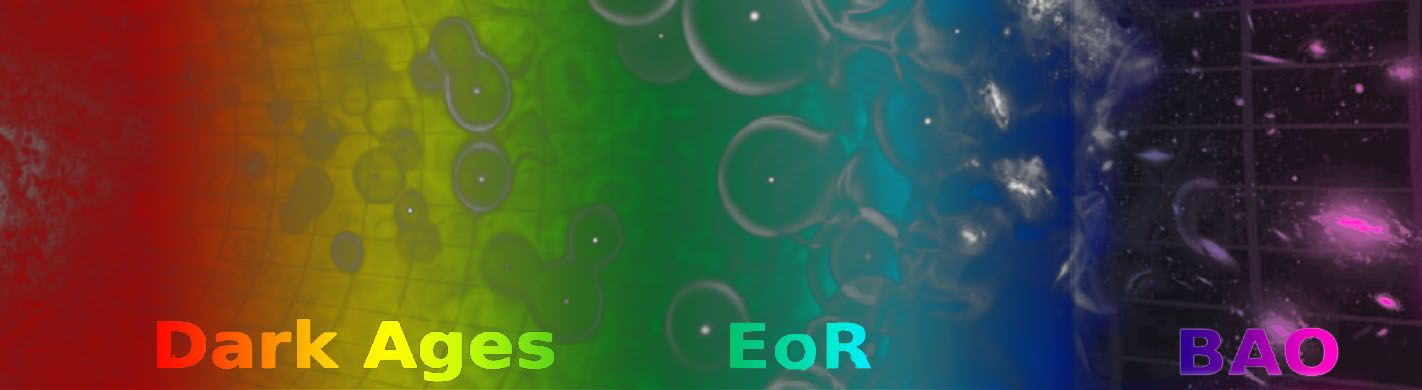
\includegraphics[height=1.25in]{plots/21cm_cosmo.jpg}
\caption{\small
Following recombination (left edge), the brightness temperature
of 21cm emission is sensitive to the density and temperature of the IGM
through the Dark Ages ($z\!\sim$120--20), evolves with the heating and
ionization of the IGM during the Epoch of Reionization (EoR; $z\!\sim$12--6), and
traces the distribution of galaxies as the universe expands ($z<4$),
leading up the the present day (right edge).  Color indicates
the redshifting of the 21cm line between 50 MHz (red) and 1.4 GHz (violet).
}\label{fig:21cm_cosmo}
\end{figure}

As large scale structures in the IGM grow through gravitational
instability and are heated and ionized by luminous sources, fluctuations
are introduced in 21cm emission (see Figure \ref{fig:21cm_cosmo}).  
Imaging of these fluctuations is a long-range goal, but in the short term, statistical
measurements (such as the power spectrum shown in Figure \ref{fig:eor_pspec}) may be more powerful.  
%Figure
%\ref{fig:eor_pspec} shows how the power spectrum of 21cm fluctuations
%evolves through a fiducial reionization model. 
Fluctuations decrease in amplitude 
as the gas is heated in the first stages of
reionization, then increase as large ionized bubbles form around galaxies, and finally fade again
as the majority of the gas is ionized.
Variations in the ultraviolet and
X-ray backgrounds, in addition to the normal density fluctuations in the IGM,
induce additional structure in the 21cm background. These fluctuations, from the Dark Ages
through reionization, are the primary target of HERA. Measuring them allows us to
probe the properties of high$-z$ galaxies and how they affected the Universe
around them.  Specifically, HERA will help us understand when reionization
occurred, how the cosmic web evolved, where the first generation of quasars
formed, when the first galaxies formed, and what their properties were.

\vspace{-0.25in}
\section{Experimental Approach}

The challenges facing 21cm reionization experiments are daunting.  
Such experiments require unprecedented levels of sensitivity, and
the brightness temperatures of foregrounds, in the form of
galactic synchrotron emission, continuum point-sources, and polarized
galactic/extra-galactic emission, exceed the fluctuations of the 21cm signal by
more than 5 orders of magnitude
\citep{santos_et_al2005,pritchard_loeb2012,pober_et_al2013b}.
%Such
%experiments require unprecedented levels of sensitivity, instrumental
%calibration, and foreground characterization.  The spectral response of these
%instruments is of paramount importance; it is used both for constructing the
%line-of-sight direction of 3D space, and also for differentiating
%smooth-spectrum foreground emission from spatial fluctuations in the
%cosmological signal. 
These foregrounds are proving very difficult to attack
head-on.  The need for sensitivity drives experiments toward
using interferometers, but the frequency-dependent instrumental
response of antenna cross-correlations 
causes what are otherwise smooth-spectrum foregrounds to 
appear with spectral structure that mimics the variation expected from 21cm reionization.
Approaches adopted by LOFAR and the MWA aim to use extremely accurate models of
foreground and instruments to
remove such chromatic effects.  However, this is proving to be a
challenging and costly task, and it remains uncertain whether this approach is
practically viable given realistic limitations on calibration accuracy.

\begin{figure}[!ht]\centering
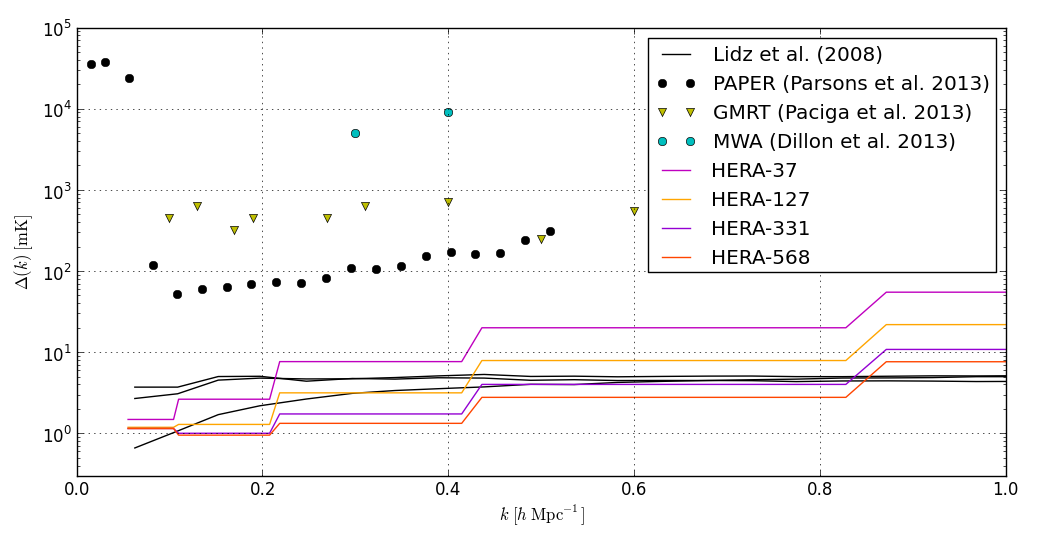
\includegraphics[height=2.75in]{plots/eor_pspec.png}
\caption{\small
$2\sigma$ upper limits on the 21cm EoR power spectrum at $z\sim8$, along
with fiducial signal models for several ionization fractions (black;
\citealt{lidz_et_al2008}),
and the predicted RMS sensitivies of HERA in various stages, including sample variance
and baseline-dependent foreground cutoffs.
The foreground isolation in PAPER measurements
above $k\approx0.1h\ {\rm Mpc}^{-1}$
are a testament to the crucial role that instrument design
plays in mitigating foreground systematics.
}\label{fig:eor_pspec}
\end{figure}

PAPER has made significant progress following a different approach.  Based on a
``delay-spectrum'' understanding of the mechanism for how instrumental
responses modulate foregrounds on spectral scales of cosmological interest
\citep{parsons_et_al2012b}, PAPER has optimized its instrument to focus on
regions in Fourier space that have weak coupling to foregrounds. 
These regions are determined both
by chromatic instrumental responses and by the inherent frequency structure of
the foregrounds.
In order to access these regions, PAPER employs antenna elements with smooth
spectral responses and uses compact antenna configurations to minimize
instrumental chromaticity.
Observations based on
this new approach are demonstrating that the extremely stringent level of
foreground removal needed to access the 21cm signal is largely in hand 
(as shown in Figure \ref{fig:eor_pspec}), with
upper limits that are beginning to rule out cold reionization scenarios. 

\vspace{-0.25in}
\section{Project Plan and Timeline}

\begin{figure}[!ht]\centering
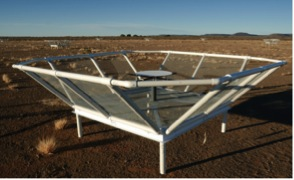
\includegraphics[height=1.75in]{plots/paper_element.jpg}
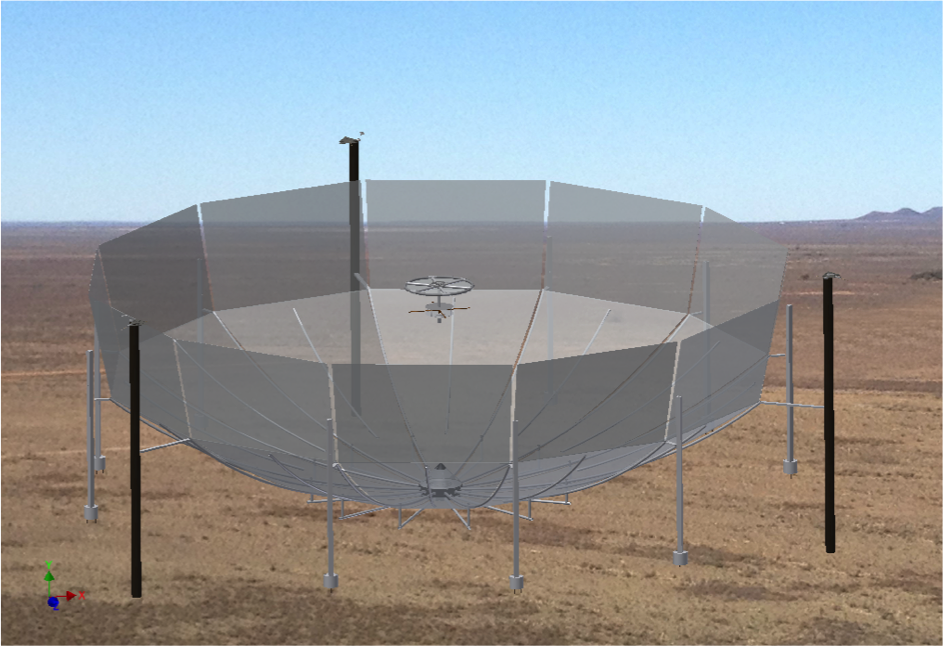
\includegraphics[height=1.75in]{plots/hera_dish.png}
\caption{\small
The PAPER element (left) provides a clean instrumental response as a function
of frequency \citep{parsons_et_al2010,parsons_et_al2012b}, which is crucial to
the foreground isolation shown in Figure \ref{fig:eor_pspec}.  A 14m dish
designed around the same feed (right) dramatically improves sensitivity while
constraining the path length and amplitude of
reflections to ensure that foreground isolation is not substantially degraded.  
}\label{fig:hera_dish}
\end{figure}

This HERA proposal targets a 568-element array that incorporates these proven
foreground avoidance techniques while addressing the sensitivity limitations of
current experiments.  With a new understanding of how antenna size and
separation affect sensitivity and foreground isolation, it
has become evident a revision of the PAPER design can yield up to 30
times the sensitivity per element without substantially degrading
foreground isolation.  Where PAPER's elements lack collecting area and are
smaller than strictly required for foreground isolation, and the majority of
MWA and LOFAR elements are spaced too widely to avoid foregrounds, HERA employs
an extremely compact array of 14m parabolic dishes with PAPER-style dipole
feeds (see Figure \ref{fig:hera_dish}.
The short (4.5m) focal height of these
dishes is central to limiting the path length of reflections whose time-delay
gives rise to chromatic instrumental systematics. 

The size of HERA dishes optimizes cost for a fixed sensitivity and level
of foreground isolation.  The associated reduction in the number of antenna
elements, combined with the fact that these dishes have no moving parts, are
built from inexpensive materials, and follow a simple construction that can be
delegated to local contractors, makes the cost of building HERA's Phase-II
experiment several times cheaper than was anticipated in the roadmap
submitted to NWNH.  
HERA follows a staged build-out plan similar to that championed by PAPER.  In
each deployment stage, improvements are incorporated into the system, and new
science capabilities are unlocked.  This approach has the advantage of
providing early access to science, permitting longer development times for
certain system components, and reducing the project risk by testing systems
early and changing them incrementally.  As shown in Figure \ref{fig:eor_pspec}, each
stage of HERA brings an associated improvement in sensitivity that allow key
aspects of 21cm reionization science to be addressed.  The timeline of HERA
development, along with the associated science products, is outlined below. 

{\bf Year 1 (FY 2015)}.  Develop
infrastructure (ground leveling, power, basic network connectivity) at
a new `K3' site $\sim$10 km from the current PAPER site
in South Africa.  Upon completion of PAPER-128
observations in Apr. 2015, migrate PAPER antennas,
correlator, and EMC container to the K3 site, and combine
with 37 hexagonal-packed prototype HERA dishes based on existing PAPER feeds and
electronics. Students, engineers, and local interns handle physical
construction.  Begin development activities
for improving HERA baluns, receivers, node electronics, and feeds from PAPER
designs.  Begin exploratory development of {\it in situ} antenna calibration subsystems,
the spatial FFT correlator, and the various software analysis pipelines.

{\bf Year 2 (FY 2016)}.  Perform HERA-37 commissioning observations, 
along with 91 PAPER elements, using the existing PAPER correlator.
Verify HERA dish performance; calibrate beam
patterns against PAPER beam responses; check for problematic
spectral structure from reflections.  Perform science observations
Oct. 2015 to Apr. 2016 that, because HERA-37 has $\sim$10 times the sensitivity of
PAPER-128, have a high probability of
detecting the peak levels of the 21cm EoR power spectrum.   Finish site
infrastructure (high-bandwidth optical network, surveying, trenching).
Finalize and fabricate improved HERA feeds and receivers in Jan.  2016.
Local contractors handle
physical construction (trenching, pole installation, assembly) of
a 127-element HERA array featuring new feeds and a refined dish design,
replacing existing 37 elements.  

{\bf Year 3 (FY 2017)}.  Perform HERA-127 
science observations from Oct. 2016 to Apr. 2017 using the PAPER correlator.
Publish HERA-37 science papers.   Finalize and fabricate node and correlator designs.
Analyze the HERA-127 dataset to constrain the timing
and duration of reionization.  Contractors expand HERA-127 to a 331-element array
from May to Sep.
Install node electronics in the field and a new
GPU correlator in an off-site building,
with optical links carrying digitized data.
Install data storage infrastructure.  Upgrade the UPenn data analysis cluster.

{\bf Year 4 (FY 2018)}.  Perform HERA-331 science observations from 
Oct. 2017 to Apr. 2018.  Publish HERA-127 results.
Fabricate nodes and antenna parts. Analyze HERA-331
dataset to characterize 
the slope of the power spectrum and distinguish between 
sources of ionizing photons.  Deploy HERA-568, following the same
Year 3 pattern.  Optionally repurpose FX correlator hardware 
for the spatial FFT correlator, with real-time calibration.

{\bf Year 5 (FY 2019)}.  Perform HERA-568 science observations from Oct. 2018
to Apr. 2019.  Publish HERA-331 results.  
Prepare and test final imaging and power-spectrum software pipelines. 
Analyze the HERA-568 dataset to produce images of bright EoR structures,
and extend power-spectrum analysis to lower frequency bands.

%\section{Broader Impacts and Benefit to the Community}
\vspace{-0.25in}
\section{Project Management Plan}

This project strikes a balance between the light-weight
management structure of HERA-I activities and the more formal structure
required for larger-scale projects.  Building on PAPER's excellent track record
and the resources of UC Berkeley's Radio Astronomy Laboratory (RAL),
this proposal consolidates responsibility and management of the core HERA
fabrication and construction activities at RAL. Parsons serves as
Project Director/Scientist; DeBoer serves as Project Manager/Engineer.
Executive 
(Aguirre, Bradley, Hewitt, Morales, Werthimer) 
and Scientific (Aguirre, Bowman, Carilli, Hewitt, Morales, Tegmark) Advisory Boards advise Parsons.
Site Manager Goeke (MIT) supervises and manages
construction activities executed by local contractors at the South African
site, and reports to DeBoer.  SKA-SA Liason Walbrugh (supported by SKA-SA)
interacts with Goeke, DeBoer and the SKA-SA board to
coordinate HERA and SKA site activities.

An external advisory board evaluates the baseline design 
based on existing components in a Preliminary Design Review at project inception.
A Critical Design Review in Year 3 evaluates the 
production design, incorporating improvements to the analog system
and feeds (Bradley), the node and correlator (Werthimer), and the data storage
system (Aguirre).
Software development, calibration, power-spectral analysis, and imaging responsibilities 
are shared across institutions, coordinated at NRAO, MIT, UCB, and U. Washington,
respectively.
Fabrication of electronics systems 
is contracted to, e.g., Digicom Technologies; antenna
component fabrication is contracted to, e.g., Burns Industries, 
including delivery to site.  Construction on site proceeds
with 2-3 teams of local contractors and laborers, managed by Goeke.  As with
PAPER, observing proceeds autonomously without local observers; SKA-SA
provides occasional site support as necessary.

Project risk and contingency are handled primarily by de-scoping.  Baseline designs using
existing hardware establish a low-risk path to basic functionality.  Improved functionality
results from successful development activities or is otherwise de-scoped.
Cost excesses and schedule slips are absorbed by reducing
build-out, with associated de-scoping of science capabilities.

%\begin{table}
%\label{tab:params}
%\begin{tabular}{|l|rl|l|}
%\hline
%Parameter & Value & Units & Description \\
%\hline
%$N$  &  576  & & Number of Antennas \\
%$d$ & 14 & m & Antenna Diameter \\
%$f/d$ & 0.32 &  & Focal Length (fractional) \\
%$\Omega_{\rm P}$ & 0.026 & sr & Field of View (power) \\
%$\Omega_{\rm PP}$ & 0.013 & sr & Field of View (power$^2$) \\
%$\Omega_{\rm eff}$ & 0.052 & sr & Field of View (sensitivity) \\
%$B_{\rm samp}$ & 0--250 & MHz & Sampled Frequency Range \\
%$B_{\rm corr}$ & 100 & MHz & Correlated Bandwidth \\
%Config.	& 24 $\times$ 24 & & Square Grid Antenna Configuration\\
%$f/f_0$ & $1.5\cdot10^5$ & & Redundancy Metric (Parsons et al. 2012a) \\
%$A$ & 0.09 & km$^2$ & Total Collecting Area \\
%$\theta$ & 15 & arcmin & Angular Resolution (150 MHz) \\
%$b_{\rm max}$ & 500 & m & Maximum Baseline \\
%$T_{\rm sys}$ & 500 & K & System Temperature \\
%$t_{\rm obs}$ & 120 & days & Observing Time \\
%$t_{\rm day}$ & 6 & hrs & Observing Time Per Day\\
%$\Delta_{\rm N}^2$ & 1.6 & mK$^2$ & Expected Noise Level ($k=0.2 h\ {\rm Mpc}^{-1}$) \\
%SNR$_{21}$ & 11.7$\sigma$ &  & Expected Detection Significance (Lidz et al. 2008, $x_i=0.5$, 150 MHz) \\
%\hline
%\end{tabular}
%\end{table}

\clearpage
\setcounter{page}{1}
\thispagestyle{empty}
%\bibliographystyle{apj}
%\bibliographystyle{hapj}
\bibliographystyle{jponew}
\bibliography{biblio}


\end{document}

